\section{Multi-weight} \label{sec:intro}


\begin{table}
\begin{tabular*}{\columnwidth}{|l|p{0.76\columnwidth}|}
\hline
\bf Symbol		& \bf Meaning \\\hline
$G\mathbf{(V,E)}$ 	& A graph with node set $V$ and edge set $E$ \\\hline 
$v_i$			& A node in $V$ \\\hline 
$(v_i,v_j)$		& An edge in $E$ \\\hline 
$\omega_k(v_i,v_j)$	& The edge weight of $(v_i,v_j)$ using weight category $\varsigma_k \in \mathcal{W}$ \\\hline
$\mathcal{W}$		& Set of possible weight categories $\mathcal{W}$, where $\varsigma_k$ denotes the category $k$ \\\hline

$Q_{s,t,w}$		& \spath query from node $v_s$ to node $v_t$, using weight $w$\\\hline
$P_{s,t,w}$		& The \spath result of $Q_{s,t,w}$ \\\hline
$|P_{s,t,w}|$		& The size of $P_{s,t,w}$ (in number of nodes) \\\hline
$E_{s,t,w}$		& The expense of executing query $Q_{s,t,w}$ \\\hline
$\chi_{s,t,w}$		& The frequency of a \spath with weight type w \\\hline
$\Psi$ 			& The Cache \\\hline
$\mathfrak{U}^w(P_{s,t,w})$& The set of all subpaths in $P_{s,t,w}$ \\\hline
$\mathfrak{U}^w(\Psi)$	& The set of all subpaths of paths in $\Psi$ \\\hline
$\gamma^w(\Psi)$		& The total benefit of the content in the cache \\\hline

$d_{s,t,w}$		& The \spath distance of a path $P_{s,t,w}$ \\\hline
$\mathcal{QL}^w$		& Query log of search queries \\\hline
\end{tabular*}
\caption{Table of Symbols \textbf{MW}}
\label{tab:symbols}
\end{table}

% 
% 
% \begin{algorithm}[bht]
% \dontprintsemicolon
% \SetVline
% 
% \SetKwInOut{Input}{input}\SetKwInOut{Output}{output}\SetKw{Return}{return}
% 
% \Input{
% 
% 	$(q,R)$: A Range query\;
% 	$\mathcal{O}$: A set of POI \;
% }
% 
% \Output{
% 
% 	A set \poi $\in \mathcal{O}$ \;
% }
% 
% \funcc{Fair}{(q,R), \mathcal{O}}
% {
%     \ForEach{$o_i \in \mathcal{O} : \mathfrak{d}_{q,o_i} \leq R$}
%     {
%       $candidate_{\mathcal{O}} \leftarrow o_i$ \;
%     }
%     result $\leftarrow$ \naivens((q,R), $candidate_{\mathcal{O}}$) \;
% 
%     \Return{result} \;
% }
% 
% \caption{Fair Algorithm}
% \label{alg:fair}
% \end{algorithm}


In multi-weight road networks\cite{icdeMouratidisLY10} a shortest path query may be submitted to a service provider based on different shortest path metrics or categories. A category could be the fastest route, the fewest number of edges to traverse, or of cause the actual shortest distance. These kind of queries require the \spath service provider to have several weights defined for each edge, a fair assumption on most service providers (TODO: CITE).
Such queries present a challenge to effectively cache, as the same \spath $P_{s,t,w}$ may not be valid for all weights/metrics $w$.
Two queries with identical start- and end-point can return two different \spathsns, depending on what weight category is issued with the query. Figure \ref{fig:map1} shows a map with two weight categories on each edge, $w_1,w_2$. The two queries $Q_{1,6,w_1}$ \& $Q_{1,6,w_2}$ are identical, except for the weight category. $\psi_1$ and $\psi_2$ in table \ref{tab:expsi} show the \spath result of the two queries in column "cache item". It is clear that the result of the two queries are very different because of the difference in weight category used for each result.




\begin{definition}
Let $G(V, E)$ be a graph with a set $V$ of nodes and a set $E$ of edges.
Each node $v_i \in V$ models a road junction. Each edge $(v_i, v_j) \in
E$ models a road segment. The weight or 'length' of an edge is denoted as $W(v_i, v_j, w)$, where $w \in \mathcal{W}$ is the weight type (length, travel time, scenic value, ect.).
\end{definition}



\begin{definition}{Multi-weight Search}\\
A Multi-weight Search query, denoted by $Q_{s,t,w}$ consist of a source and target vertex $s$ and $t$, plus a category $w \in \mathcal{W}$ 
The result of $Q_{s,t,w}$, denoted $P_{s,t,w}$, is a collection of connected vertices $v_s,\dotsc,v_t$ such that they form a \spath on graph $G\mathbf{(V,E)}$ using category $w \in \mathcal{W}$.
\end{definition}


Using the map1 (fig. \ref{fig:map1}) a multi-weight search query, $Q_{1,2,w}$, can be executed for two different weights, $w_1$ or $w_2$, possibly resulting in two different paths for the same start-/end-nodes, depending on the weight chosen. Table \ref{tab:expsi} shows the \spath $\psi_1$ and $\psi_2$ resulting from the same start-/end-node, but using different weights ($w_1, w_2$).


\begin{figure}[hbt]
  \center
        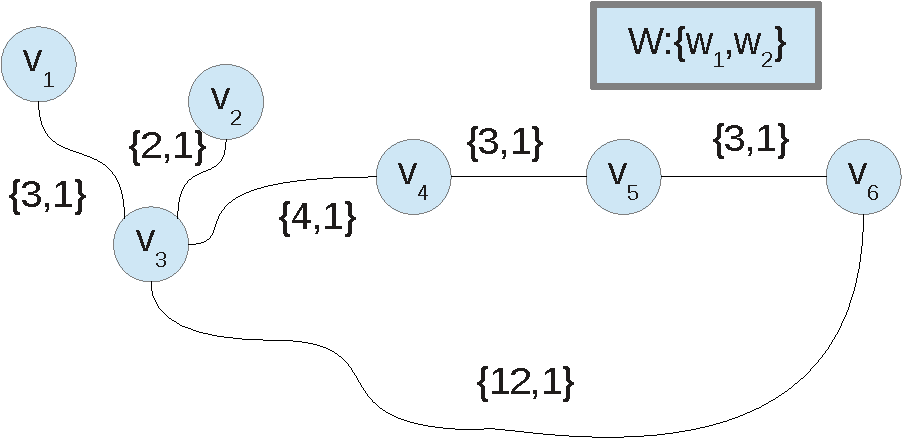
\includegraphics[width=0.4\textwidth]{figures/map1}
        \caption{Map1. Has a set of two weights on each edge, $w_1,w_2$.}
  \label{fig:map1}
\end{figure}

\begin{table}
\begin{tabular}{l|l|l}\hline
$\psi$		& Cache item 			& Category \\\hline  \hline
$\psi_1:$	& $\{v_1,v_3,v_4,v_5,v_6\}$ 	& ($w_1$)\\\hline
$\psi_2:$	& $\{v_1,v_3,v_6\}$ 		& ($w_2$)\\\hline
$\psi_3:$	& $\{v_1,v_3,v_4,v_5\}$ 	& ($w_1,w_2$)\\\hline
\end{tabular}
\caption{Cache items using queries $Q_{1,6,X}, Q_{1,5,X}$ with $X:\{w_1,w_2\}$, covering both weights on the map (fig \ref{fig:map1})}
\label{tab:expsi}
\end{table}


\begin{definition}{Multi-weight Query Log ($\mathcal{QL}^{w}$)}\\
A multi-weight search query log $\mathcal{QL}^w$ is a collection of time stamped queries that have been issued by users in the past.
A query is on the form $(s,t,w)$, where $s$ and $t$ is the start- and end-point respectively. $w$ is the category to be used when calculating the SP. The full form of the log, $\mathcal{QL}^{w}$,  is then: $\{(s_0,t_0,w_0),\dots,(s_i,t_i,w_i)\}$.
\end{definition}



\subsection{Cache Structure}

Paths are stored as sets of vertices $\{(s_0,t_0),\dots,(s_i,t_i)\}$ with an associated category $w \in W$ in the cache. Instead of using a single inverted list to look up whether the cache can answer a query, we use a collection of inverted lists to keep track of which $Q_{s,t,w}$ can be answered by the cache ($\Psi$), for each category in $\mathcal{W}$.
Even if a full path can only answer a query for a single weight type, then by using this approach then any sub-path able to answer for more than one weight-type will still be utilized. 

The map in figure \ref{fig:map1} depicts a simple road system with 2 different weights on each edge. The first edge weight captures edge length, while the second weight captures the of number of edges traversed, which is why each edge always contributes 1.

To answer a query $Q_{s,t,w}$ on the cache in table \ref{tab:expsi}, for each item $\psi_i$, we first check whether $w$ matches any of the entries in the category column. If $w$ matches an entry we then we check whether $s \in \psi_i$ and $t \in \psi_i$, if yes, then $\psi_i$ can answer $Q_{s,t,w}$. We search each entry in the table until either we find an match, or all entries have been examined.

If we want to answer the query $Q_{1,4,w_2}$ we will first check the category column of $\psi_1$, as it does not include $w_2$ we know it can not answer our query and we proceed to check $\psi_2$. Since $\psi_2$ can answer some query with category $w_2$ we check whether $v_1 \in \psi_2$ and $v_4 \in \psi_2$. Since $v_4 \not \in \psi_2$ we proceed to check $\psi_3$. As the category of $\psi_3$ contains $w_2$ and $v_1, v_4 \in \psi_3$ we know that $\psi_3$ can answer $Q_{1,4,w_2}$.

As the cache in table grows larger it becomes inefficient to search, so we extend the idea of using inverted list from \cite{thomsen2012}(sec. 4.2). Assuming the following four historical queries, \\
$Q_{1,6,w_1},Q_{1,6,w_2}, Q_{1,5,w_1},Q_{1,5,w_2}$ from $\mathcal{QL}^{w}$, we will have the cache items in table \ref{tab:expsi}. Using this we build a inverted list for each weight in order to quickly answer queries (see fig. \ref{fig:wilist}). 
To answer a query $Q_{v_s,v_t,w}$ we use $w$ to first find the relevant inverted list. Afterwards we do 2 look-ups in the inverted list, for $v_s$ \& $v_t$ respectively, and then check the intersection of the cache items. If the answer is non-empty there is a \spath for $Q_{v_s,v_t,w}$ in the cache. 
A more efficient approach would be to combine all the tables together and make the key (weight,vertex). This would reduce the number required lookups to two, and since the tables most likely will have some identical items, then we may also have a chance to optimize the number of entries.

\begin{figure}[hbt]
  \center
        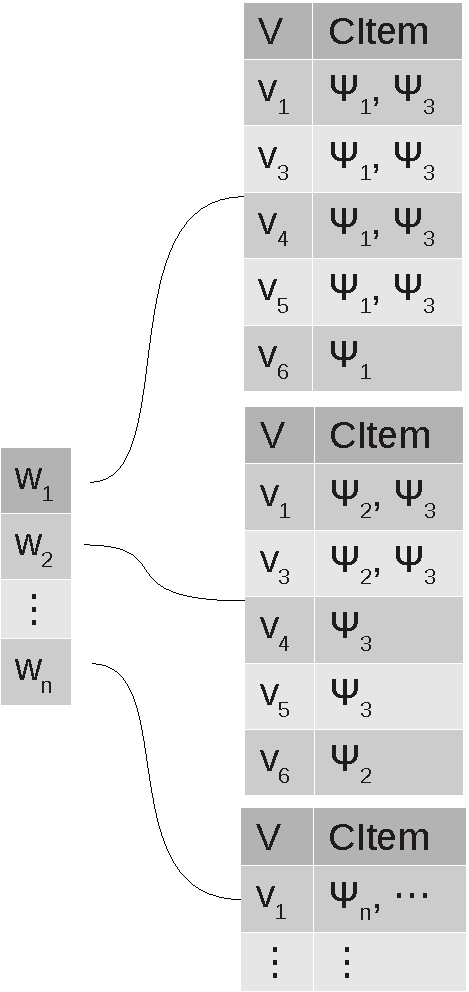
\includegraphics[width=0.20\textwidth]{figures/wilist}
        \caption{Cache structure for inverted lists using map1 (fig. \ref{fig:map1}) and cache elements from table \ref{tab:expsi}}
  \label{fig:wilist}
\end{figure}

\subsection{Benefit Model}

We extend the benefit driven benefit model introduced in \cite{thomsen2012}. We introduce what changes are needed to capture the benefit of \spaths with \textit{multi-weight search}.
Equation \ref{eq:phiw}, \ref{eq:benefitw}, \ref{eq:upsw}, and \ref{eq:cachebenefitw} define the existing functions with restriction on $w$.


We have to answer two important questions:
\begin{enumerate}
\item \label{quest:impone} Which queries $Q_{s,t,w}$ can be answered by the path $P_{s,t,w}$?
\item \label{quest:imptwo} For query $Q_{s,t,w}$ what is the benefit if added to the cache.
\end{enumerate}

Question \ref{quest:impone} can be answered by the updated lemma \ref{lem:weightedoptimalproperty} (from \cite{thomsen2012}). A path $P_{a,b,d}$ contains the path $P_{s,t,w}$ if they share the same weight and both $v_s$ \& $v_t$ are on $P_{a,b,d}$. With this we get the updated definition for the \textit{answerable query set}, $\mathfrak{U}^w(P_{a,b,d})$, for path $P_{a,b,d}$:

\begin{equation} \label{eq:phiw}
\mathfrak{U}^w(P_{a,b,d}) = \{ P_{s,t,w} : s, t \in P_{a,b,d},  s \neq t,  d = w\}
\end{equation}

Equation \ref{eq:phiw} finds all sub-paths of SP $sp$ with weight category $w$. Using cache item $\psi_1$ from $Q_{v_1,v_6}$ in table \ref{tab:expsi}, the answerable queryset is: $\mathfrak{U}^w(P_{1,6,w_1}) = \{P_{1,3,w_1},P_{1,4,w_1},P_{1,5,w_1},P_{1,6,w_1},P_{3,4,w_1},$ $P_{3,5,w_1},P_{3,6,w_1},P_{4,5,w_1},P_{4,6,w_1},P_{5,6,w_1}\}$ 


In regards to question \ref{quest:imptwo} we update the \textit{benefit} equation $\gamma(\Psi)$ to consider weight categories:

\begin{equation} \label{eq:benefitw}
\gamma^w(P_{a,b,d}) = \sum\limits_{P_{s,t,w} \in \mathfrak{U}^w(P_{a,b,d})} \chi_{s,t,w} \bullet E_{s,t,w}
\end{equation}

Equation \ref{eq:benefitw} defines $benefit$ and makes it clear how much can we expect to save, in total, if path $P_{a,b,d}$ is in the cache. It is calculated based on the historical statistics defined by $\chi_{a,b,d}$ (equation \ref{eq:chiw}) and the cost of calculating the \spathns, $E_{a,b,d}$.


\begin{equation} \label{eq:chiw}
\chi_{s,t,w} =  |\{ Q_{b,e,w} \in \mathcal{QL}^{w}: s, t \in Q_{b,e,w} \}|
\end{equation}

\begin{equation} \label{eq:chiSingleToRegw}
 \hat{\chi}_{R_i, R_j, w} = \sum\limits_{v_s \in R_i} \sum\limits_{v_t \in R_j} \chi_{s,t,w}
\end{equation}


\begin{equation} \label{eq:chiregw}
\chi_{s,t,w} = \frac{ \hat{\chi}_{R_i, R_j, w} }{|R_i| \cdot |R_j|}
\end{equation}



Based on how often we have seen the path, and its subpaths, in the query log $\mathcal{QL}^{w}$, equation \ref{eq:chiw} defines the benefit of a path, for a single path. Equation \ref{eq:chiSingleToRegw} for $\hat{\chi}_{R_i, R_j, w}$ sums up all $\chi_{s,t,w}$ going from a vertex $v_s$ in region $R_i$ to a vertex $v_t$ in $R_j$. Using equation \ref{eq:chiSingleToRegw} we can then define $\chi_{s,t,w}$ for regions as equation \ref{eq:chiregw}.




\begin{lemma} \label{lem:weightedoptimalproperty}
\textbf{Weighted optimal subpath property} (modified from \cite{thomsen2012}, Lemma 1)\\

The \spath $P_{a,b,d}$ contain the \spath $P_{s,t,w}$ if $v_s \in P_{a,b,d}, v_t \in {P_a,b,d}$ and $d = w$, where $d,w \in \mathcal{W}$
Let $P_{a,b,d}$
Specifically, let $P_{a,b,d} = \langle v_{x_0},v_{x_1},v_{x_2},...,v_{x_m}\rangle$. 
We have $P_{s,t,w} = \langle v_{x_i},v_{x_i+1},...,v_{x_j}\rangle$ if $v_s = v_{x_i}, v_t = v_{x_j}$, and $w = d$ for some i,j such that $0 \leq i \leq j \leq m$
\end{lemma}



For the general case where the cache contains more than one path, the updated equations are shown below:

\begin{equation} \label{eq:upsw}
 \mathfrak{U}^w(\Psi) = \bigcup\limits_{P_{a,b,w} \in \Psi} \mathfrak{U}^w(P_{a,b,d})
\end{equation}

Equation \ref{eq:upsw} finds the set of unique paths with weight $w$ from $\Psi$, which is either a path from $a$ to $b$, or a sub-path of such a path. This is the answerable set of paths using  $P_{a,b,d}$.

\begin{equation} \label{eq:cachebenefitw}
\gamma^w(\Psi) = \sum\limits_{P_{s,t,w} \in \mathfrak{U}^w(\Psi)} \chi_{s,t,w} \cdot E_{s,t,w}
\end{equation}

Equation \ref{eq:cachebenefitw} calculate the benefit of the cache with respect to a specific weight category, using $\chi_{s,t,w}$ and $E_{s,t,w}$, in the same way $\chi_{s,t}$ is calculated using $\chi_{s,t}$ and $E_{s,t}$.





The same query with different weight can result in different cache items. In table \ref{tab:expsi} the queries $Q_{1,6,w_1},Q_{1,6,w_2} \in \mathcal{QL}^{w}$, the two only differing on the weight parameter. The two queries results in both $\psi_1$ and $\psi_2$ being in the cache, since the query returns two different paths for weights $w_1$ and $w_2$. 
It can of cause also be the case that no matter what weight we use, the \spath is the same. The queries $Q_{1,5,w_1},Q_{1,5,w_2} \in \mathcal{QL}^{w}$ are an example of this, as the \spath does not change for $w_1$ or $w_2$. 
An important aspect to notice is that though a complete cache item may only valid for a single weight category, then a sub path of the \spath can be valid for several categories. This can e.g. be seen in $\psi_1$ (table \ref{tab:expsi}) where the path is only valid for $w_1$, but $\psi_1 \setminus v_6$ is identical to $\psi_3$ which we already know is valid for both $w_1,w_2$. Avoiding this duplication of information could e.g. be done by using inverted lists as in fig. \ref{fig:wilist} to store the information on weight category. If we do so we will not need to store $\psi_3$, since $\psi_3 \in \psi_1$.





% 
% \begin{tabular}{|l|l|}\hline
% \textbf{V} &	\textbf{Cache Item} \\\hline
% $V_1$	&	$\psi_1, \psi_3$ \\\hline
% $V_3$	&	$\psi_1, \psi_3$ \\\hline
% $V_4$	&	$\psi_1, \psi_3$ \\\hline
% $V_5$	&	$\psi_1, \psi_3$ \\\hline
% $V_6$	&	$\psi_1$ \\\hline
% \end{tabular}
% \vspace{2em}
% 
% \begin{tabular}{|l|l|}\hline
% \textbf{V} &	\textbf{Cache Item} \\\hline
% $V_1$	&	$\psi_2, \psi_3$ \\\hline
% $V_3$	&	$\psi_2, \psi_3$ \\\hline
% $V_4$	&	$\psi_3$ \\\hline
% $V_5$	&	$\psi_3$ \\\hline
% $V_6$	&	$\psi_2$ \\\hline
% \end{tabular}

\section{Direction Assistance}


\begin{table}
\begin{tabular*}{\columnwidth}{|l|p{0.76\columnwidth}|}
\hline
\bf Symbol		& \bf Meaning \\\hline
$G\mathbf{(V,E)}$ 	& A graph with node set $V$ and edge set $E$ \\\hline 
$v_i$			& A node in $V$ \\\hline 
$(v_i,v_j)$		& An edge in $E$ \\\hline 

$Q_{s,t}$		& \spath query from node $v_s$ to node $v_t$\\\hline
$P_{s,t}$		& The \spath result of $Q_{s,t}$. \\\hline
$|P_{s,t}|$		& The size of $P_{s,t}$ (in number of nodes) \\\hline
$E_{s,t}$		& The expense of executing query $Q_{s,t}$ \\\hline
$\chi_{s,t}$		& The frequency of a \spath \\\hline
$\Psi$ 			& The Cache \\\hline
$\mathfrak{U}(P_{s,t})$& The set of all subpaths in $P_{s,t}$ \\\hline
$\mathfrak{U}(\Psi)$	& The set of all subpaths of paths in $\Psi$ \\\hline
$\gamma(\Psi)$	& The total benefit of the content in the cache \\\hline

$d_{s,t}$		& The \spath distance of a path $P_{s,t}$ \\\hline

$\mathcal{QL}$		& Query log of search queries (see \cite{thomsen2012}) \\\hline
\end{tabular*}
\caption{Table of Symbols \textbf{DA}}
\label{tab:symbols}
\end{table}

When looking for directions to some place, a user who issues a \spath query does not actually care about the full \spathns\cite{sigmodTaoSP11}, but rather the user just wants to know when a new action is needed (turn left, right, or any action other action, besides following the current path. This is what GPS devices usually do. GPS devices usually only alerts the user if an action is needed, otherwise the user should just continue on the current path.
There are two extremes when calculating directions for a \spathns:

\begin{tabular}{@{}l@{  } p{21em} }
Fine ({\bf F})		& The directions are given for every single node on the \spathns, regardless of whether there are any option to change directions. \\
Coarse ({\bf C})	& The directions are given only when it is necessary to change directions, i.e. it does not matter how many side roads are passed, as long as the instruction is ostensibly "continue straight", then the instruction will not be included. Only if it is really necessary to make an action, such as turning, will the node be included in the instructions.
\end{tabular}

Both $fine$ and $coarse$ will always include the start- and end-node. There are many possible alternatives to the two extremes, as they represent the maximum ({\bf F}) and minimum ({\bf C}) number of nodes a \spath can be recorded with. Any alternative $(\textbf{A}):(\textbf{C}) \subseteq (\textbf{A}) \subseteq (\textbf{F})$ is possible. 
One possible alternative (\textbf{A}) could be to have the directions be given only for nodes where it is possible to change direction/turn and we will be using this alternative in figure \ref{tab:psilvlcontent} and \ref{tab:directioninvlists}. 

The same query can be saved at many different levels of detail, figure \ref{fig:minroute} shows a route from S to T, where each node on the route is marked as necessary for a $fine$\textbf{(F)} and/or $coarse$\textbf{(C)} level of detail. Table \ref{tab:psilvlcontent}, $\psi_1$, shows the set of nodes included in the path from $v_1$ to $v_{11}$, depending on whether the level of detail is set as \textbf{(F),(C)}, or a mix \textbf{(A)}. It is important to note that the end user will always be satified with \textbf{(C)}, and that the option of saving a full path \textbf{(F)} or something between the two \textbf{(A)} is decided at the service providers side to tweak the performance of the \spath cache.


When using (\textbf{F}) the advantage is that all subpaths of a \spath in the cache will be answerable, this scheme may however take op a lot of space for subpaths that will never be part of a query answer, and therefor contribute no benefit to the cache.

Using (\textbf{C}) the advantage is that, especially on longer \spathsns, it will consume less space, while still maintaining enough information in the cache, enabeling it to answer some sub-queries, assuming the result includes some actions. The downside is of cause that the reduced number of vertices stored also negatively impacts the number of queries that can be answered by the \spath when it is in the cache.

It may be desireble to use some alternative (\textbf{A}) to gain the benefit of being able to answer more paths than a cache item found with (\textbf{C}) allows for, and at the same time not have to store any nodes that we do not consider useful (according to equation \ref{eq:benefitl} and \ref{eq:cachebenefitl}).


In figure \ref{fig:minroute} a path from S to T is shown. Each vertex is labeled based on what level of directions each node would be included in, according to the enumeration of (\textbf{F}) and (\textbf{C}) above. No alternative \textbf{A}) is shown on the map.


\begin{figure}[hbt]
  \center
        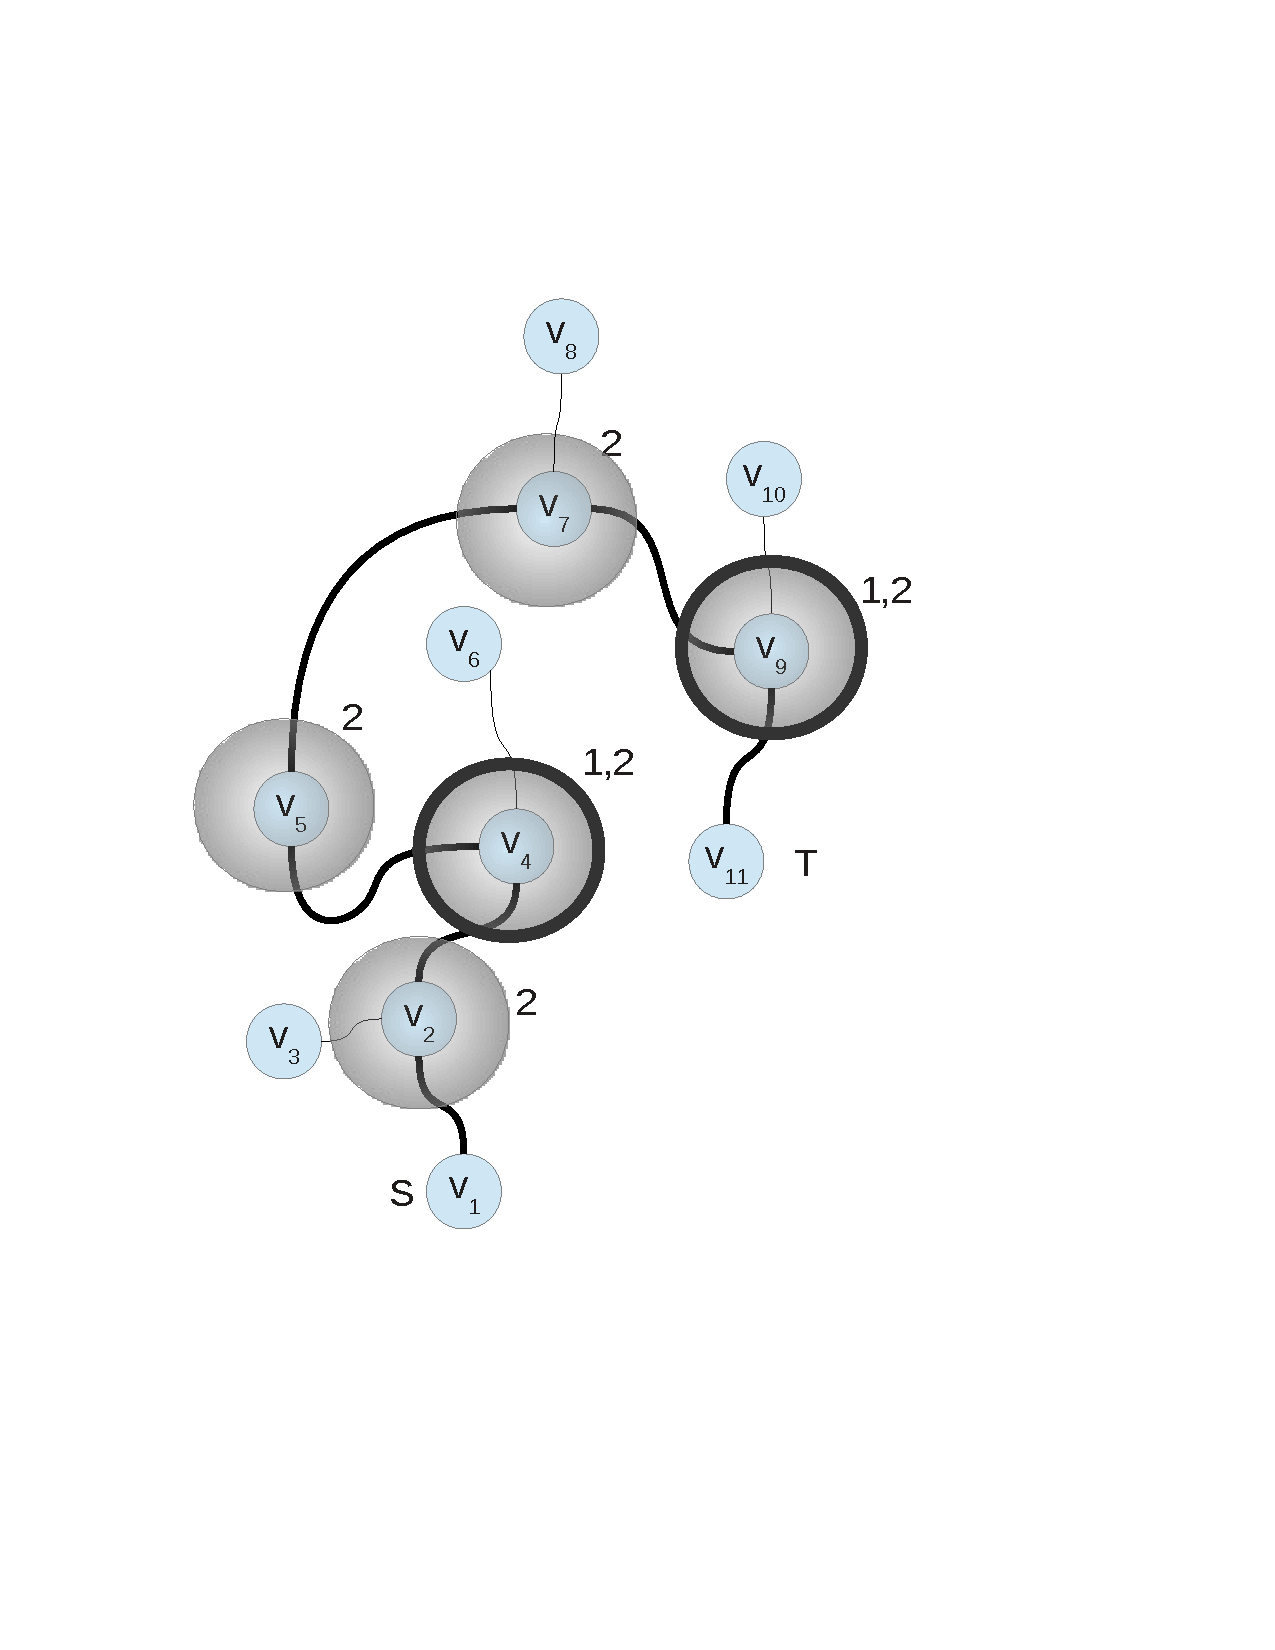
\includegraphics[width=0.4\textwidth]{figures/minroute}
        \caption{$Q_{1,11}$: Bold line from S to T denote travel route. (\textbf{F}): All nodes on the path has an (F), forming the complete path. 
        (\textbf{C}): Circles with a (C) denote the minimum set of nodes needed to navigate from S to T}
  \label{fig:minroute}
\end{figure}


\begin{definition}\label{def:direction} {Direction}\\
The \textit{directions} of a query $Q_{s,t}$, where the detail level $l$ is specified by (\textbf{F}), (\textbf{C}), and some an Alternative(\textbf{A}):(\textbf{C}) $\leq$ (\textbf{A}) $\leq$ (\textbf{F}) , are a set of vertex neighbour pairs $\{(v_s,v_i),...,(v_j,v_k),...,(v_l,v_t)\}$, each pair consisting of two connected nodes on $P_{s,t}$, representing a instruction at a node $v_j$, to take the path towards node $v_k$, where$v_j,v_k \in V$ on the \spath $P_{s,t}$.
$l$ is a system parameter set by the service provider.
\end{definition}

Figure \ref{fig:minroute} illustrates the $directions$ on query $Q_{1,11}$ for level being set to both (\textbf{C}) and (\textbf{F}). For (\textbf{F}) the $directions$ include the all vertices on the bold path from S to T. For (\textbf{C}) the $directions$ only include the circled vertices: The start- and end-vertex plus a pair of neighbouring nodes each time the default action of going straight needs to be changed because the path turns where there are more than one choice.

\begin{definition}
Let $G(V, E)$ be a graph with a set $V$ of nodes and a set $E$ of edges.
Each node $v_i \in V$ models a road junction. Each edge $(v_i, v_j) \in
E$ models a road segment. The weight (length) of an edge is denoted as $W(v_i, v_j)$.
\end{definition}


\begin{definition}{\spathns: Query and Result}\\
A shortest path query, denoted by $Q_{s,t}$ consist of a source and target node, $v_s,v_t$.

The result of $Q_{s,t}$, denoted $P_{s,t}$, is a collection of nodes on the \spath from $v_s$ to $v_t$ (on the graph G) with, as minimum, a pair of nodes for each action to take (definition \ref{def:direction}).
We can represent $P_{s,t}$ as a list of pairs (node, neighbour node): $\langle (v_{s},v_{x_{}}), (v_{x_1},v_{x_{1n}}), \dots ,(v_{x_n},v_{x_{nn}}) \rangle$, where each pair contains a set of neighbouring vertices from $G$.
\end{definition}




\subsection{Cache Structure}

Cache items can be stored just as they did before \cite{thomsen2012}, either in a path array or as a graph representation. 

Table \ref{tab:directioninvlists} shows the inverted lists for different detail levels, based the cache content in table \ref{tab:psilvlcontent} and the map from figure \ref{fig:minroute}. Table \ref{tab:directioninvlists} shows the tables as three separate tables, there is however no reason they could not be combined, so different keys, $v_i$, point to the same data.

Figuring out at what detail level paths should be stored in the cache, and whether the should be stored in a path array or as a graph representation is one of the interesting questions we want to answer. 

For longer \spaths that are relatively simple, meaning few instructions are needed, we will store very few nodes at level (\textbf{C}). This could be a problem as we have no information about how to traverse large parts of such a shortest path, even if such parts may be have high benefit (high $\chi$ values for pairs of nodes on the path). We could possibly use the $\chi$ benefit values to determine how many extra vertices we have to store besides the ones at level (\textbf{C}). One such alternative is to simply calculate the result of all queries in $\mathcal{QL}$ and then simply union any resulting path which is fully a subpath of another path (example in section \ref{subsec:benmod}). This would allow us to store only the nodes that are both necessary and useful for navigation.


\begin{table}
\begin{tabular}{@{}l@{}l@{}|@{}l@{}|@{}l@{}|@{}l@{}|@{}}\cline{3-5}
			&		& \bf \;(F)				& \bf \;(C)			& \bf \;(A) \\\cline{3-5}
$Q_{1,11}$		& ($\Psi_1$)	& $v_1,v_2,v_4,v_5,v_7,v_8,v_9,v_{11}$ 	& $v_1,v_4,v_5,v_9,v_{11}$ 	& $v_1,v_2,v_4,v_5,v_9,v_{11}$\\\cline{3-5}
$Q_{3,8}$		& ($\Psi_2$)	& $v_3,v_2,v_4,v_5,v_7,v_8$		& $v_3,v_2,v_4,v_5,v_8$ 	& $v_3,v_2,v_4,_5,v_8$\\\cline{3-5}
$Q_{2,6}$		& ($\Psi_3$)	& $v_2,v_4,v_6$				& $v_2,v_6$			& $v_2,v_4,v_6$\\\cline{3-5}
\end{tabular}
  \caption{Example of how cache items will look when executed at different detail level}
  \label{tab:psilvlcontent}
\end{table}

\begin{table}
\begin{tabular}{c c c}
  \begin{tabular}{l|l|}\cline{2-2}
		  & \bf (F)			 \\\cline{2-2}
  $v_1$		& $\Psi_1$			 \\\cline{2-2}
  $v_2$		& $\Psi_1,\Psi_2,\Psi_3$	 \\\cline{2-2}
  $v_3$		& $\Psi_2$			 \\\cline{2-2}
  $v_4$		& $\Psi_1,\Psi_2,\Psi_3$	 \\\cline{2-2}
  $v_5$		& $\Psi_1,\Psi_2$		 \\\cline{2-2}
  $v_6$		& $\Psi_3$			 \\\cline{2-2}
  $v_8$		& $\Psi_1,\Psi_2$		 \\\cline{2-2}
  $v_9$		& $\Psi_1$			 \\\cline{2-2}
  $v_{11}$	& $\Psi_1$			 \\\cline{2-2}
  \end{tabular}
&
  \begin{tabular}{l|l|}\cline{2-2}
		  & \bf (C)			 \\\cline{2-2}
  $v_2$		& $\Psi_1,\Psi_2,\Psi_3$	 \\\cline{2-2}
  $v_4$		& $\Psi_1,\Psi_2,\Psi_3$	 \\\cline{2-2}
  $v_9$		& $\Psi_1$			 \\\cline{2-2}
  \end{tabular}
&
  \begin{tabular}{l|l|}\cline{2-2}
		  & \bf (\textbf{A})		 \\\cline{2-2}
  $v_2$		& $\Psi_1,\Psi_2,\Psi_3$	 \\\cline{2-2}
  $v_4$		& $\Psi_1,\Psi_2,\Psi_3$	 \\\cline{2-2}
  $v_5$		& $\Psi_1,\Psi_2$		 \\\cline{2-2}
  $v_8$		& $\Psi_1,\Psi_2$		 \\\cline{2-2}
  $v_9$		& $\Psi_1$			 \\\cline{2-2}
  \end{tabular}
   \\
   (a)	& (b)	& (c)
\end{tabular}
        \caption{Inverted lists for (\textbf{F}),(\textbf{C}), and (\textbf{A})}
  \label{tab:directioninvlists}
\end{table}


\subsection{Benefit model}\label{subsec:benmod}

The benefit model of \cite{thomsen2012} is extended to work with directions to make it clear how we define benefit in this
scenario. $\chi_{s,t,l}$ (equation \ref{eq:chil}) and $E_{s,t,l}$ are defined as in \cite{thomsen2012}. Except for the introduction and restriction on level, there is no not much difference in the benefit equations. 


Saving \textbf{(F)} in the cache all the time will most likely waste cache space, as some nodes will never be needed to answer any query. Storing \textbf{(C)} all the time will save space and allow for more items in the cache, they will however only be able to answer very specific queries. Clearly the best choice is to choose some \textbf{(A)}, remember $(\textbf{C}) \subseteq (\textbf{A}) \subseteq (\textbf{F})$. The challenge is then to figure out $which$ \textbf{(A)} to save in the cache to achive maximum benefit, using the least amount of cache space. 

To give an intuitive example of how such an \textbf{(A)} may be found we use the example paths shown in figure \ref{fig:altmap}. The example paths are found using a liniar map, where \textbf{Map} is the longest possible path in this example. As a map like this precludes the possibility of turns, it is clear that if we save paths at the granularity of \textbf{(C)}, then only the start- and end-point needs to be saved. However, when looking at path this The simple nature of the map clearly illustrates that if we were to add the the start-/end-points from A to F to the cache, we would be duplicating information several times. When trying to add path A to the cache we can find the set of other paths which are also subpaths of A. In figure \ref{fig:altmap} this set consist of path C,D, and E. Instead of adding the start-/end-points of path C,D,E directly to the cache as seperate cache items, we can simply added their nodes as internal nodes of A, so A is can now be stored as A$_{alt}: \{1,3,4,6\}$. Since C,D, and E all share node 4, plus C and E share their end node with A, then such an alternative would save 4 nodes less in the cache. Since we would originally have used 8 nodes to store A,C,D,E in the cache, we achive a reduction of 50\% in space consumption. Equation \ref{eq:optPath} illustrates how to find one such union of paths, when starting with a path $P_{s,t}$. 



\begin{equation}\label{eq:optPath}
O_{a,b} = \{s,t : P_{s,t} \in \mathfrak{U}_l(P_{a,b}),  Q_{s,t} \in \mathcal{QL}\}
\end{equation}


Our problem then becomes how to choose the path $O_{s,t}$ with the maximum benefit to the cache.

Finding the most beneficial $O_{s,t}$ can be done by finding  $sp = |\{(P_{a,b}| : P_{s,t} \in P^{(F)}_{a,b},  Q_{s,t} \in \mathcal{QL}\}$, and finding $max(\mathfrak{U}(sp))$ from possible paths.






\begin{figure}[hbt]
  \center
        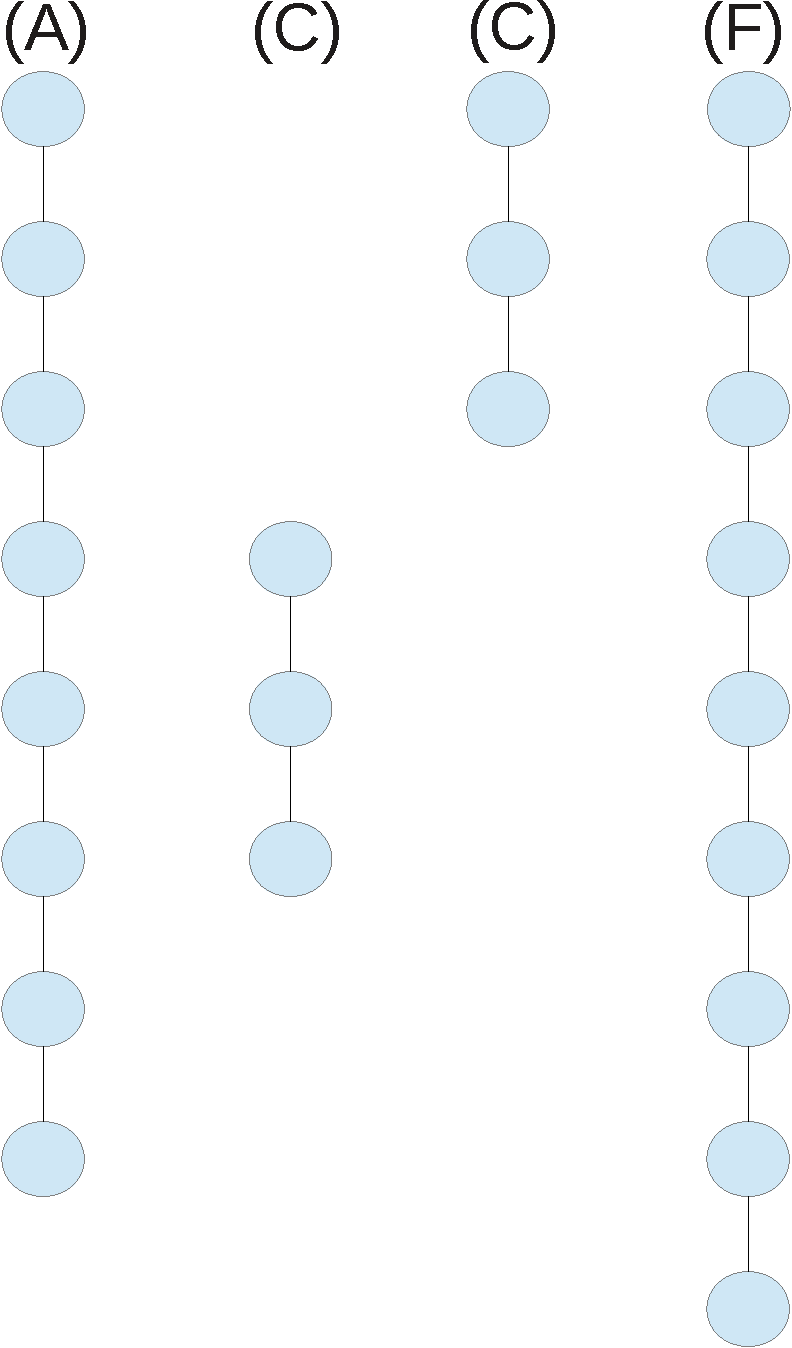
\includegraphics[width=0.4\textwidth]{figures/altmap}
        \caption{Liniar map with path A-F shown at \textbf{(C)} granularity. A$_{alt}$ shows the union of path A,C,D,E.}
  \label{fig:altmap}
\end{figure}







Below equation \ref{eq:phil}, \ref{eq:benefitl}, \ref{eq:upsl}, and \ref{eq:cachebenefitl} are briefly described, they are identical to the the equations in \cite{thomsen2012}. Equation \ref{eq:chil} does not appear in \cite{thomsen2012}, however, the definition is identical.

\begin{equation} \label{eq:phil}
\mathfrak{U}(P_{a,b}) = \{ P_{s,t} : s, t \in P_{a,b},  s \neq t\}
\end{equation}

Equation \ref{eq:phil} finds all sub-paths of $P_{a,b}$. When using directions at the coarsest level \textbf{(C)},  we will not be able to answer as many subpaths from the path $P_{a,b}$ as we originally could, equation \ref{eq:phil} captures this reduction in value as the \textit{answerable query set} will be smaller.


\begin{equation} \label{eq:benefitl}
\gamma(P_{a,b}) = \sum\limits_{P_{s,t} \in \mathfrak{U}(P_{a,b})} \chi_{s,t} \cdot E_{s,t}
\end{equation}

Using equation \ref{eq:phil} and \ref{eq:chil}, equation \ref{eq:benefitl} captures the benefit of adding a single path to the cache.

\begin{equation} \label{eq:chil}
\chi_{s,t} =  |\{ Q_{b,e} \in \mathcal{QL}: s, t \in Q_{b,e} \}|
\end{equation}


\begin{equation} \label{eq:upsl}
 \mathfrak{U}(\Psi) = \bigcup\limits_{P_{a,b} \in \Psi} \mathfrak{U}(P_{a,b})
\end{equation}

Equation \ref{eq:upsl} finds the set of unique paths that $P_{a,b}$, and subpaths of it, can answer from the cache. With this we are able to answer how much value a new path can add to the cache, given the items already present in the cache.

\begin{equation} \label{eq:cachebenefitl}
\gamma(\Psi) = \sum\limits_{P_{s,t} \in \mathfrak{U}(\Psi)} \chi_{s,t} \cdot E_{s,t}
\end{equation}

Equation \ref{eq:cachebenefitl} calculate the benefit of the cache.






% \section{Misc. Ideas } 

% 
% %Intro
% 
% %Equations
% 
% %Definitions
% 
% %explanation
% 
% %Figures
% 
%  \subsection{Sharing Paths}
% It might be possible to use several cache items to assist answering a query.:
% By analyzing the map it would be possible to identify junctions such as $v_3$ in \ref{fig:map1}, where any path going to/from $v_1$ or $v_2$ must pass through $v_3$. This would let us do a search in the cache for a partial result, meaning we would have to calculate a smaller \spath. This kind of search would require the \spath algorithm to have a minimum of awareness of whether a junction node could be helpful, though that could be as simple as checking whether the node lies between the x and/or y values of the source and destination of the query.
